\maketitle
\tableofcontents
\newpage

\section{Zielsetzung}
Wie geschildert in \cite{anleitung} so ist es.

\section{Theorie}
%\begin{equation}
%  \vec{B}(\vec{r}) = \frac{\mu_0}{4\pi} \int_V \vec{\jmath}(\vec{r}) \times \frac{\vec{r}-\vec{r'}}{\lvert \vec{r} - \vec{r'} \rvert^3} \ \symup{d}V'
%  \label{gleichung1}
%\end{equation}
\section{Aufbau und Durchführung}
  Siehe \eqref{gleichung1}
  \subsection{Aufbau}
  \subsection{Durchführung}
\newpage

\section{Auswertung}
\SI{27.23(1)e3}{\meter\per\second}
\begin{equation}
  \SI{27.23(1)e3}{\meter\per\second}
\end{equation}
Wie in \cite[4]{hallo} zu sehen, gibt es krasse Bizepse.
\begin{figure}
    \centering
    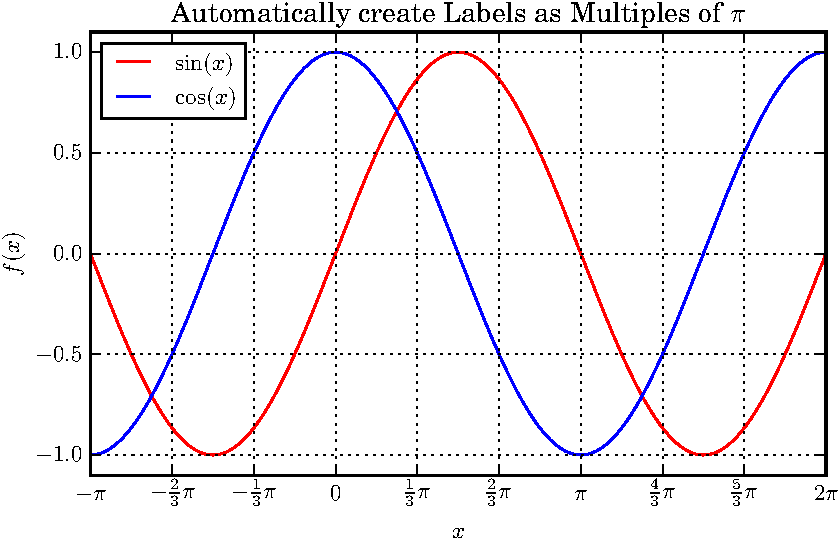
\includegraphics[width=\textwidth]{plot1.pdf}
    \caption{Automatically create Labels as Multiples of $\pi$.here are three font options which affects different parts of the caption: One affecting the
font=
labelfont=
textfont=
whole caption (
font
), one which only affects the caption label and separator (
label
-
font
) and at least one which only affects the caption text (
textfont
).  You set them
up using the options.}
    \label{fig:plot1}
\end{figure}
$0,2$ und $\num{0,2}$
$10000$ und $\num{10000}$
$3,1415926$ und $\num{3,1415926}$
\begin{gather}
  \SI{511}{\kilo\electronvolt} \\
  \SI{1e-10}{\metre} \\
  \SI{10}{\kilo\gram\meter\per\second\squared} \\
  \SI{105.6}{\kilo\gram\per\meter\per\volt\tothe{5}\per\second}
\end{gather}
\begin{equation}
  \vec{x} = \begin{pmatrix}
  1 & -1 \\
  2 & 2
  \end{pmatrix}
  \label{gleichung2}
\end{equation}
Diese Gleichung \footnote{Beste Gleichung der Welt} findet sich nochmal unten.
Auf der nächsten Seite gibts diese Gleichung \ref{fig:plot1} zu bestaunen, auf der übernächsten diese beiden \ref{fig:2plots},
wobei \ref{fig:plot3} diese eindeutig die Schönste ist.
\newpage
\section{Diskussion}
Hallo \eqref{gleichung2}. Dann gings weiter mit \cite{buch}, da es dort um die mögliche Zukunft der Welt geht. Experten sind sich
uneinig, ob es sich um eine Dystopie oder Utopie handelt. In \cite{kent} geht es auch darum.
\begin{figure}
  \centering
  \begin{subfigure}{0.48\textwidth}
    \centering
    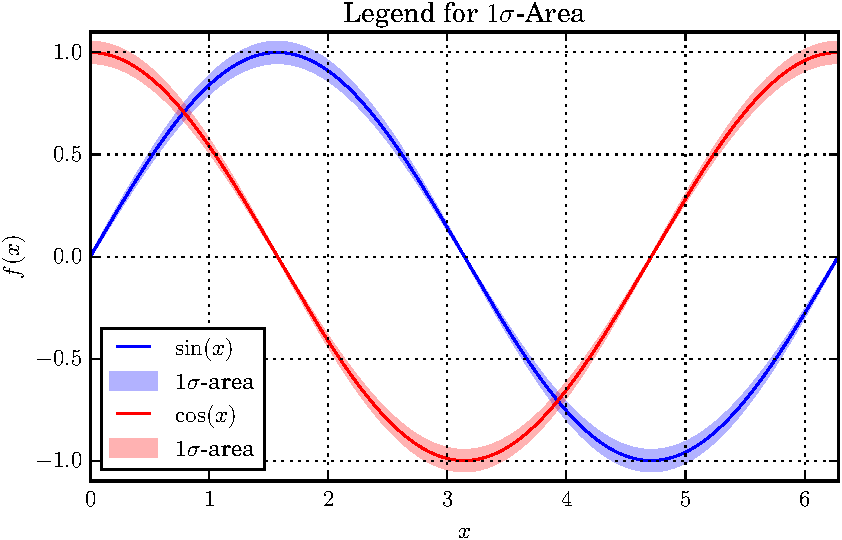
\includegraphics[width=\textwidth]{plot2.pdf}
    \caption{Plot2.}
    \label{fig:plot2}
  \end{subfigure}
    \begin{subfigure}{0.48\textwidth}
      \centering
      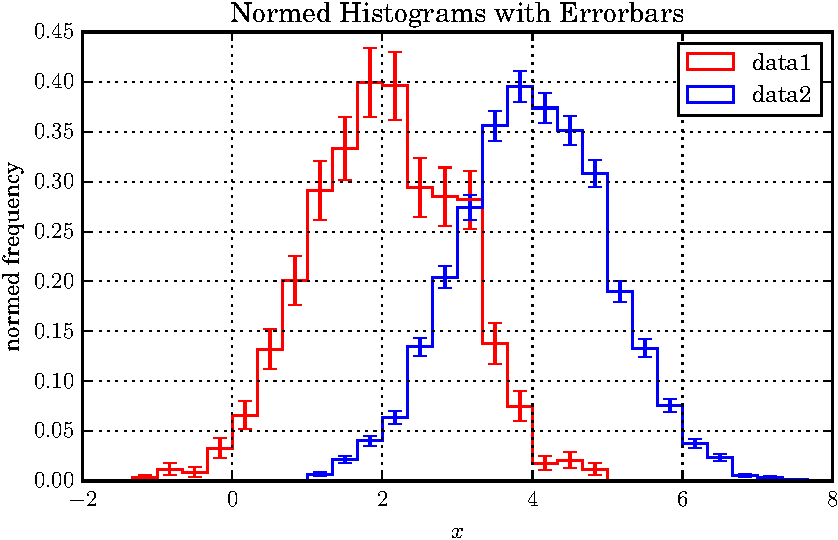
\includegraphics[width=\textwidth]{plot3.pdf}
      \caption{Plot3.}
      \label{fig:plot3}
  \end{subfigure}
  \caption{Zwei Logos, Abbildung \subref{fig:plot3}: Plot 3.}
  \label{fig:2plots}
\end{figure}
\newpage
\nocite{*}
\printbibliography
